\documentclass[twoside,twocolumn]{article}
\usepackage[hmarginratio=1:1,top=32mm,columnsep=20pt]{geometry}
\usepackage[hang, small,labelfont=bf,up,textfont=it,up]{caption} 
\usepackage{amsmath}
\usepackage{amsfonts}
\usepackage{booktabs}
\usepackage{enumitem}
\setlist[itemize]{noitemsep}
\usepackage{abstract}
\renewcommand{\abstractnamefont}{\normalfont\bfseries}
\renewcommand{\abstracttextfont}{\normalfont\small\itshape}
\usepackage{titlesec}
\renewcommand\thesection{\Roman{section}}
\renewcommand\thesubsection{\Alph{subsection}}
\renewcommand\thesubsubsection{\arabic{subsubsection}}
\titleformat{\section}[block]{\normalsize\bfseries\scshape\centering}{\thesection.}{1em}{}
\titleformat{\subsection}[block]{\normalsize\bfseries\centering}{\thesubsection.}{1em}{}
\titleformat{\subsubsection}[block]{\normalsize\centering}{\thesubsubsection.}{1em}{}
\usepackage{fancyhdr}
\pagestyle{fancy}
\fancyhead{}
\fancyhead[C]{Computational Physics Homework $\bullet$ July 2018 $\bullet$ Vol. Final, No. 1}
\usepackage{titling}
\usepackage{hyperref}
\hypersetup{unicode}
\AtBeginShipoutFirst{\input{zhwinfonts.tex}}
\usepackage{bm}
\usepackage{braket}
\usepackage{CJKutf8}
\usepackage{xcolor}
\usepackage{dcolumn}
\usepackage{graphicx}
\usepackage{indentfirst}
\usepackage{listings}
\usepackage[toc, page, title, titletoc, header]{appendix}
\definecolor{grey}{rgb}{0.8,0.8,0.8}
\definecolor{darkgreen}{rgb}{0,0.3,0}
\definecolor{darkblue}{rgb}{0,0,0.3}
\def\lstbasicfont{\fontfamily{pcr}\selectfont\footnotesize}
\lstset{
	numbers=left,
	escapeinside=``,
	numberstyle=\small,
	showstringspaces=false,
	showspaces=false,
	tabsize=4,
	frame=single,
	basicstyle={\footnotesize\lstbasicfont},
	keywordstyle=\color{darkblue}\bfseries,
	identifierstyle=,
	commentstyle=\color{darkgreen},
	stringstyle=\color{black}
}
\lstloadlanguages{C,C++,Fortran,Java,Matlab,Mathematica,Python}
\setlength{\parindent}{2em}
\begin{document}
\begin{CJK*}{UTF8}{gkai}
%----------------------------------------------------------------------------------------
%	TITLE SECTION
%----------------------------------------------------------------------------------------

\setlength{\droptitle}{-4\baselineskip} % Move the title up
\pretitle{\begin{center}\Huge\bfseries} % Article title formatting
	\posttitle{\end{center}} % Article title closing formatting
\title{计算物理期末大作业} % Article title
\author{
	\textsc{梁旭民}\thanks{\noindent 指导老师:齐新老师} \\[1ex] % Your name
	\normalsize Cuiying Hornors College, Lanzhou University \\ % Your institution
	\normalsize \href{mailto:liangxm15@lzu.edu.cn}{liangxm15@lzu.edu.cn} % Your email address
}
\date{}
\renewcommand{\maketitlehookd}{
	\begin{abstract}
		本次作业求解的是矩形导体边界接地情况下内部有一个点电荷的Poisson方程和圆形导体边界接地情况下内部有一个点电荷的Poisson方程,通过在Cartesian坐标系和极坐标系下分别生成差分格式矩阵,并处理对应的点电荷,得到了线性方程组。分别利用Gauss消元法、Jacobi迭代法、Gauss Seidel迭代法和SOR超松弛迭代法,可以解出线性方程组,即通过有限差分法求得了Poisson方程的解,不断增加了分成的格点我们可以比较不同方法求解线性方程的速度快慢。
	\end{abstract}
}
\maketitle

%----------------------------------------------------------------------------------------
%	SECTION 1
%----------------------------------------------------------------------------------------

\section{Introduction}
	Poisson方程是数学中一个常见于静电学、机械工程和理论物理的偏微分方程,因法国数学家、几何学家及物理学家Poisson而得名的。
	\subsection{方程的叙述}
	Poison方程为
	\begin{equation*}
	\Delta\varphi=f
	\end{equation*}
	在这里$\Delta$代表的是Laplace算子,而$f$和$\varphi$可以是在流形上的实数或复数值的方程。当流形属于Euclid空间,而Laplace算子通常表示为${\nabla}^2$,因此Poisson方程通常写成
	\begin{equation*}
	{\nabla}^{2}\varphi=f
	\end{equation*}
	在三维直角坐标系,可以写成
	\begin{equation*}
	\left( \frac{\partial^2}{\partial x^2} + \frac{\partial^2}{\partial y^2} + \frac{\partial^2}{\partial z^2} \right)\varphi(x,y,z) = f(x,y,z)
	\end{equation*}
	
	如果有$f(x,y,z)$恒等于$0$,这个方程就会变成一个齐次方程,这个方程称作“Laplace方程”
	\begin{equation*}
	\Delta \varphi = 0
	\end{equation*}
	
	Poisson方程可以用Green函数来求解,现在也发展出很多种数值解,如松弛法迭代法。
	\subsection{数学表达}
	通常泊松方程表示为
	\begin{equation*}
	-\Delta\varphi=f
	\end{equation*}
	这里$\Delta$代表Laplace算子,$f$为已知函数,而$\varphi$为未知函数。当$f=0$时,这个方程被称为Laplace方程。
	
	为了解Poisson方程我们需要更多的信息,比如Dirichlet边界条件: 
	\begin{equation*}
	\begin{cases}
	-\Delta \varphi =f&{\text{in}}\ \Omega \\
	\varphi =g&{\text{auf}}\ \partial \Omega
	\end{cases}
	\end{equation*}
	其中$\Omega\subset\mathbb{R}^{n}$为有界开集。
	
	这种情况下利用基础函数构建Poisson方程的解,Laplace方程的基础函数为: 
	\begin{equation*}
	\Phi (x)=
		\begin{cases}
		-{\dfrac {1}{2\pi }}\ln |x|&n=2\\
		{\dfrac {1}{n(n-2)\omega _{n}}}{\dfrac {1}{|x|^{n-2}}}&n\geq 3
		\end{cases}
	\end{equation*}
	其中$\omega _{n}$为$n$维欧几里得空间中单位球面的体积,此时可通过卷积$(\Phi *f)$得到$-\Delta \varphi =f$的解。
	
	为了使方程满足上述边界条件,我们使用Green函数
	\begin{equation*}
	G(x,y)=\Phi (y-x)-\phi ^{x}(y)
	\end{equation*}
	$\phi ^{x}$为一个校正函数,它满足
	\begin{equation*}
	\begin{cases}
	\Delta \phi ^{x}=0&{\text{in}}\ \Omega \\
	\phi ^{x}=\Phi (y-x)&{\text{auf}}\ \partial \Omega 
	\end{cases}
	\end{equation*}
	通常情况下$\phi ^{x}$是依赖于$\Omega$。
	
	通过$G(x,y)$可以给出上述边界条件的解
	\begin{equation*}
	\begin{aligned}
		u(x)=&-\int _{{\partial \Omega }}g(y){\frac {\partial G}{\partial \nu }}(x,y){\mathrm {d}}\sigma (y)\\
		&+\int _{\Omega }f(y)G(x,y){\mathrm {d}}y
	\end{aligned}
	\end{equation*}
	其中$\sigma$表示$\partial\Omega$上的曲面测度。
	
	此方程的解也可通过变分法得到。
\section{The Method}
	\subsection{问题描述}
	先通过有限差分法生成矩阵,利用消元法(或者LU法)、Jacobi迭代、Gauss Seidel迭代、超松弛(SOR)迭代分别求解矩形和圆形接地导体边界情况下,点电荷在空间中的电势分布。并不断增加矩阵尺寸,比较各种方法计算速度。其中矩形边界用Cartesian坐标系,圆形边界用极坐标系。
	\subsection{有限差分法简介}
	在数学中,有限差分法(finite-difference methods,简称FDM),是一种微分方程数值方法,是通过有限差分来近似导数,从而寻求微分方程的近似解。
	\subsubsection{由Taylor展开式的推导}
	首先假设要近似函数的各级导数都有良好的性质,依照Taylor定理,可以得到以下的Taylor展开式:
	\begin{equation*}
	\begin{aligned}
	f(x_{0}+h)=f(x_{0})&+{\frac {f'(x_{0})}{1!}}h+{\frac {f^{(2)}(x_{0})}{2!}}h^{2}+\\\cdots& +{\frac {f^{(n)}(x_{0})}{n!}}h^{n}+R_{n}(x)
	\end{aligned}
	\end{equation*}
	其中$n!$表示是$n$的阶乘,$R_{n}(x)$为余数,表示泰勒多项式和原函数之间的差。可以推导函数$f$一阶导数的近似值:
	\begin{equation*}
	f(x_{0}+h)=f(x_{0})+f'(x_{0})h+R_{1}(x)
	\end{equation*}
	设$x_{0}=a$,可得:
	\begin{equation*}
	f(a+h)=f(a)+f'(a)h+R_{1}(x)
	\end{equation*}
	除以$h$可得:
	\begin{equation*}
	{f(a+h) \over h}={f(a) \over h}+f'(a)+{R_{1}(x) \over h}
	\end{equation*}
	求解$f^{\prime}(a)$:
	\begin{equation*}
	f^{\prime}(a)={f(a+h)-f(a) \over h}-{R_{1}(x) \over h}
	\end{equation*}
	假设$R_{1}(x)$相当小,因此可以将函数$f(x)$的一阶导数近似为:
	\begin{equation*}
	f'(a)\approx {f(a+h)-f(a) \over h}
	\end{equation*} 
	\subsubsection{准确度及误差}
	近似解的误差定义为近似解及解析解之间的差值。有限差分法的两个误差来源分别是舍入误差及截尾误差(或称为离散化误差),前者是因为电脑计算小数时四舍五入造成的误差,后者则是计算机内数字位数限制造成的误差。
	有限差分法是以在格点上函数的值为准
	
	\begin{figure}[h]
	\centering
	\includegraphics[width=0.6\linewidth]{figure/figure1}
	\caption{有限差分法是以在格点上函数的值为准}
	\label{fig:figure1}
	\end{figure}
	
	在运用有限差分法求解一问题(或是说找到问题的近似解)时,第一步需要将问题的定义域离散化。一般会将问题的定义域用均匀的网格分割(见Figure 1)。因此有限差分法会制造一组导数的离散数值近似值。
	
	一般会关注近似解的局部截尾误差,会用大$O$符号表示,局部截尾误差是指应用有限差分法一次后产生的误差,因此为$f'(x_{i})-f'_{i}$,此时$f'(x_{i})$是实际值,而$f'_{i}$为近似值。Taylor多项式的余数项有助于分析局部截尾误差。利用$f(x_{0}+h)$Taylor多项式的余数项,也就是
	\begin{equation*}
	 R_{n}(x_{0}+h)={\frac {f^{(n+1)}(\xi )}{(n+1)!}}(h)^{n+1}
	\end{equation*}
	其中$x_{0}<\xi <x_{0}+h$
	
	可以找到局部截尾误差的主控项,例如用前项差分法计算一阶导数,已知$f(x_{i})=f(x_{0}+ih)$,则有
	\begin{equation*}
	f(x_{0}+ih)=f(x_{0})+f'(x_{0})ih+{\frac {f''(\xi )}{2!}}(ih)^{2}
	\end{equation*}
	
	利用一些代数的处理,可得
	\begin{equation*}
	{\frac {f(x_{0}+ih)-f(x_{0})}{ih}}=f'(x_{0})+{\frac {f''(\xi )}{2!}}ih
	\end{equation*}
	
	注意到左边的量是有限差分法的近似,右边的量是待求解的量再加上一个余数,因此余数就是局部截尾误差。上述范例可以用下式表示:
	\begin{equation*}
	{\frac {f(x_{0}+ih)-f(x_{0})}{ih}}=f'(x_{0})+O(h)
	\end{equation*}
	在此例中,局部截尾误差和时间格点的大小成正比。
	\subsection{Cartesian坐标下有限差分格式}
	Cartesian坐标下静电场的二维Poisson方程可以表示为
	\begin{equation*}
	\nabla^{2}\varphi(x,y)=\frac{\partial^{2}\varphi}{\partial x^{2}}+\frac{\partial^{2}\varphi}{\partial y^{2}}=-\frac{-\rho (x,y)}{\varepsilon_{0}}
	\end{equation*}
	\begin{figure}[h]
	\centering
	\includegraphics[width=0.9\linewidth]{figure/figure2}
	\caption{二维Cartesian坐标网络五点差分格式}
	\label{fig:figure2}
	\end{figure}
	
	在二维网格中的差分格式可以写作
	\begin{equation*}
	\begin{aligned}
	&\nabla^{2}\varphi(x_{i},y_{j})=-\frac{\rho_{i,j}}{\varepsilon_{0}}\\
	&=\frac{1}{h^{2}}(\varphi_{i-1,j}+\varphi_{i+1,j}+\varphi_{i,j-1}+\varphi_{i,j+1}-4\phi_{i,j})
	\end{aligned}
	\end{equation*}
	矩阵法是将未知量和已知量之间的线性关系表示为矩阵的形式,通过对矩阵进行消元和变换直接求出未知量的值。矩阵的边长等于总格点个数。可将矩阵表示为如下形式
	\begin{equation*}
	\left[~
	\begin{array}{c|c|c}
		\begin{matrix}
		\mathbf{B}
		\end{matrix}&
		\begin{matrix}
		e& &\\
		&\ddots&\\
		& &e
		\end{matrix}&
		\begin{matrix}
		\end{matrix}
		\\\hline
		\begin{matrix}
		d& &\\
		&\ddots&\\
		& &d
		\end{matrix}&
		\begin{matrix}
		\mathbf{\ddots}
		\end{matrix}&
		\begin{matrix}
		e& &\\
		&\ddots&\\
		& &e
		\end{matrix}
		\\\hline
		\begin{matrix}
		\end{matrix}&
		\begin{matrix}
		d& &\\
		&\ddots&\\
		& &d
		\end{matrix}&
		\begin{matrix}
		\mathbf{B}
		\end{matrix}
	\end{array}
	~\right]
	\end{equation*}
	其中,矩阵$B$与参数分别为
	\begin{equation*}
	\mathbf{B}=
	\begin{bmatrix}
	a&c&&\\
	b&\ddots&\ddots&\\
	&\ddots&\ddots&c\\
	&&b&a
	\end{bmatrix}
	\qquad \left\{
	\begin{aligned}
	&a=4\\
	&b=c=-1\\
	&d=e=-1
	\end{aligned}
	\right.
	\end{equation*}
	\subsection{极坐标下的有限差分格式}
	在极坐标系下,我们选择厚度非常小的圆柱(实际上是为了保证物理把厚度直接当1算),则有:
	\begin{equation*}
	\begin{aligned}
		&\int_{V}\frac{\rho}{\varepsilon_{0}}dV=\frac{1}{\varepsilon_{0}}(\rho_{i,j}r_{i}\Delta \theta\Delta r)\\
		&\oint\vec{E}\cdot d\vec{S}=E_{i+\frac{1}{2},j}^{r}\cdot r_{i+\frac{1}{2}}\Delta \theta-E_{i-\frac{1}{2},j}^{r}\cdot r_{i-\frac{1}{2}}\Delta \theta\\
		&+E_{i,j+\frac{1}{2}}^{\theta}\cdot \Delta r-E_{i,j-\frac{1}{2}}^{\theta}\cdot r_{i+\frac{1}{2}}\Delta r
	\end{aligned}
	\end{equation*}
	\begin{figure}[h]
	\centering
	\includegraphics[width=0.8\linewidth]{figure/figure3}
	\caption{二维极坐标网络五点差分格式}
	\label{fig:figure3}
	\end{figure}
	
	根据Gauss定理,即:
	\begin{equation*}
	\int_{V}\frac{\rho}{\varepsilon_{0}}dV=\oint\vec{E}\cdot d\vec{S}
	\end{equation*}
	又:
	\begin{equation*}
	\left\{
	\begin{aligned}
	&E_{i+\frac{1}{2},j}^{r}=-\frac{\varphi_{i+1,j}-\varphi_{i,j}}{\Delta r}\\
	&E_{i-\frac{1}{2},j}^{r}=-\frac{\varphi_{i,j}-\varphi_{i-1,j}}{\Delta r}\\
	&E_{i,j+\frac{1}{2}}^{\theta}=-\frac{\varphi_{i,j+1}-\varphi_{i,j}}{r_{i}\Delta \theta}\\
	&E_{i,j-\frac{1}{2}}^{\theta}=-\frac{\varphi_{i,j}-\varphi_{i,j-1}}{r_{i}\Delta \theta}
	\end{aligned}\right.
	\end{equation*}
	可以得到非原点处的五点差分公式:
	\begin{equation*}
	\begin{aligned}
	&-\frac{\rho_{i,j}}{\varepsilon_{0}}=\frac{1}{r_{i}^{2}\Delta\theta^{2}}(\varphi_{i,j+1}-2\varphi_{i,j}+\varphi_{i,j-1})\\
	&+\frac{1}{r_{i}\Delta r^{2}}\left(\varphi_{i+1,j}r_{i+\frac{1}{2}}-2\varphi_{i,j}r_{i}+\varphi_{i-1,j}r_{i-\frac{1}{2}}\right)\\
	&=-\left(\frac{2}{r_{i}^{2}\Delta\theta^{2}}+\frac{2}{r_{i}\Delta r^{2}}\right)\varphi_{i,j}+\frac{r_{i+\frac{1}{2}}}{r_{i}\Delta r^{2}}\varphi_{i+1,j}\\
	&+\frac{r_{i-\frac{1}{2}}}{r_{i}\Delta r^{2}}\varphi_{i-1,j}+\frac{1}{r_{i}^{2}\Delta \theta^{2}}\varphi_{i,j+1}+\frac{1}{r_{i}^{2}\Delta\theta^{2}}\varphi_{i,j-1}
	\end{aligned}
	\end{equation*}
	对于坐标原点,同样可以解得其差分公式为
	\begin{equation*}
	\frac{\rho_{0}}{\varepsilon_{0}}=\frac{2\Delta \theta}{\pi\Delta r^{2}}\sum_{j=1}^{N_{\theta}}(\varphi_{1,j}-\varphi_{0})
	\end{equation*}
	矩阵$A$可以表示为
	\setlength{\arraycolsep}{3pt} 
		\begin{equation*}
		\left[~
		\begin{array}{c|c|c|c}
		\begin{matrix}
		m
		\end{matrix}&
		\begin{matrix}
		n \ldots n
		\end{matrix} &
		\begin{matrix}
		\end{matrix}&
		\begin{matrix}
		\end{matrix}\\\hline
		\begin{matrix}
		d_{1}\\
		\vdots\\
		d_{1}
		\end{matrix}&
		\begin{matrix}
		\mathbf{B}
		\end{matrix}&
		\begin{matrix}
		e_{1}& &\\
		&\ddots&\\
		& &e_{1}
		\end{matrix}&
		\begin{matrix}
		\end{matrix}
		\\\hline
		\begin{matrix}
		\end{matrix}&
		\begin{matrix}
		d_{2}& &\\
		&\ddots&\\
		& &d_{i}
		\end{matrix}&
		\begin{matrix}
		\mathbf{\ddots}
		\end{matrix}&
		\begin{matrix}
		e_{2}& &\\
		&\ddots&\\
		& &e_{i}
		\end{matrix}
		\\\hline
		\begin{matrix}
		\end{matrix}&
		\begin{matrix}
		\end{matrix}&
		\begin{matrix}
		d& &\\
		&\ddots&\\
		& &d
		\end{matrix}&
		\begin{matrix}
		\mathbf{B}
		\end{matrix}
		\end{array}
		~\right]
		\end{equation*}
		其中矩阵$B$和各项系数为
	\begin{equation*}
	\mathbf{B}=
	\begin{bmatrix}
	a_{i}&c_{i}&&b_{i}\\
	b_{i}&\ddots&\ddots&\\
	&\ddots&\ddots&c_{i}\\
	b_{i}&&b_{i}&a_{i}
	\end{bmatrix}
	\end{equation*}
	\begin{equation*}
	\left\{
	\begin{aligned}
	&a_{i}=\frac{2}{\Delta r^{2}}+\frac{2}{r_{i}^{2}\Delta\theta^{2}}\\
	&b_{i}=c_{i}=-\frac{1}{r_{i}^{2}\Delta\theta^{2}}\\
	&d_{i}=-\frac{r_{i-\frac{1}{2}}}{r_{i}\Delta r^{2}}\qquad e_{i}=-\frac{r_{i+\frac{1}{2}}}{r_{i}\Delta r^{2}}\\
	&m=\frac{2N_{\theta}\Delta \theta}{\pi\Delta r^{2}}\qquad n=-\frac{2\Delta}{\pi\Delta r^{2}}
	\end{aligned}
	\right.
	\end{equation*}
	\subsection{Gauss消元法}
	数学上,Gauss消元法是线性代数中的一个算法,可用来为线性方程组求解,求出矩阵的秩,以及求出可逆方阵的逆矩阵。该方法以数学家Karl Gauss命名,但最早出现于中国古籍《九章算术》,成书于约公元前150年。由于Gauss消元法在线性代数课程中为最基本的算法,这里只做简单分析:
	
	Gauss消元法的算法复杂度是$O^(n3)$;这就是说,如果系数矩阵的是$n\times n$,那么Gauss消元法所需要的计算量大约与$n^{3}$成比例。
	
	Gauss消元法可以用在电脑中来解决数千条等式及未知数。不过,如果有过百万条等式时,这个算法会十分费时。一些极大的方程组通常会用迭代法来解决。亦有一些方法特地用来解决一些有特别排列的系数的方程组。
	
	Gauss消元法可用在任何域中。
	
	Gauss消元法对于一些矩阵来说是稳定的。对于普遍的矩阵来说,Gauss消元法在应用上通常也是稳定的,不过亦有例外。
	\subsection{Jacobi迭代法}
	在数值线性代数中,Jacobi迭代法是一种解对角元素几乎都是各行和各列的绝对值最大的值的线性方程组的算法。求解出每个对角元素并插入近似值。不断迭代直至收敛。这个算法是雅可比矩阵的精简版。方法的名字来源于德国数学家Kerl Jacobi。
	\subsubsection{数学描述}
	给定一个$n\times n$的线性方程组
	\begin{equation*}
	A\mathbf{x}=\mathbf{b}
	\end{equation*}
	其中:
	\begin{equation*}
	A={\begin{bmatrix}a_{11}&a_{12}&\cdots &a_{1n}\\a_{21}&a_{22}&\cdots &a_{2n}\\\vdots &\vdots &\ddots &\vdots \\a_{n1}&a_{n2}&\cdots &a_{nn}\end{bmatrix}}
	\end{equation*}
	\begin{equation*}
	\mathbf {x} ={\begin{bmatrix}x_{1}\\x_{2}\\\vdots \\x_{n}\end{bmatrix}},\qquad \mathbf {b} ={\begin{bmatrix}b_{1}\\b_{2}\\\vdots \\b_{n}\end{bmatrix}}
	\end{equation*}
	
	$A$可以分解成对角部分$D$和剩余部分$R$:
	\begin{equation*}
	A=D+R
	\end{equation*}
	其中
	\begin{equation*}
	D={\begin{bmatrix}a_{11}&0&\cdots &0\\0&a_{22}&\cdots &0\\\vdots &\vdots &\ddots &\vdots \\0&0&\cdots &a_{nn}\end{bmatrix}}
	\end{equation*}
	\begin{equation*}
	R={\begin{bmatrix}0&a_{12}&\cdots &a_{1n}\\a_{21}&0&\cdots &a_{2n}\\\vdots &\vdots &\ddots &\vdots \\a_{n1}&a_{n2}&\cdots &0\end{bmatrix}}
	\end{equation*}
	
	线性方程组可以重写为:
	\begin{equation*}
	D\mathbf{x}=\mathbf{b}-R\mathbf{x}
	\end{equation*}
	
	Jacobi法是一种迭代方法。在每一次迭代中,上一次算出的x被用在右侧,用来算出左侧的新的x。这个过程可以如下表示:
	\begin{equation*}
	\mathbf {x} ^{(k+1)}=D^{-1}(\mathbf {b} -R\mathbf {x} ^{(k)})
	\end{equation*}
	对每个元素可以用以下公式:
	\begin{equation*}
	 x_{i}^{(k+1)}={\frac {1}{a_{ii}}}\left(b_{i}-\sum _{j\neq i}a_{ij}x_{j}^{(k)}\right),\quad i\in \mathbb{N}_{+}
	\end{equation*}
	
	注意计算$x_{i}^{(k+1)}$需要$x^{(k)}$中除了自己之外的每个元素。 不像Gauss Seidel迭代,我们不能用 $x_{i}^{(k+1)}$覆盖$x^{(k)}$,因为在接下来的计算中还要用到这些值。这是雅可比和高斯-塞德尔方法最显著的差别,也是为什么前者可以用并行算法而后者不能的原因。最小需要的存储空间是两个长度为$n$的向量。
	\subsubsection{算法描述}
	选择一个初始猜想值$x^{0}$
	\begin{equation*}
	\begin{aligned}
	&\text{while 未收敛}\\
	&\quad for~i:=1~step~until~n~do\\
	&\qquad \sigma=0\\
	&\qquad for~j:=1~step~until~n~do\\	
	&\qquad \quad if~j!=i~then\\
	&\qquad \qquad \sigma =\sigma +a_{ij}x_{j}^{(k-1)}\\
	&\qquad \quad end~if\\
	&\qquad end (j-loop)\\
	&\qquad x_{i}^{(k)}={{\left({b_{i}-\sigma }\right)} \over {a_{ii}}}\\
	&\quad end (i-loop)\\
	&\quad \text{检查是否收敛}\\
	&\text{end (未收敛时继续循环)}
	\end{aligned}
	\end{equation*}
	\subsubsection{收敛}
	标准的收敛情况是当迭代矩阵的谱半径
	\begin{equation*}
	\rho (D^{-1}R)<1
	\end{equation*}
	
	保证收敛的条件是矩阵A为严格或不可约地对角占优矩阵。严格的行对角占优矩阵指对于每一行,对角线上的元素之绝对值大于其余元素绝对值的和,即
	\begin{equation*}
	\left|a_{ii}\right|>\sum _{j\neq i}{\left|a_{ij}\right|}
	\end{equation*}
	有时即使不满足此条件,Jacobi法仍可收敛。 
	\subsection{Gauss Seidel迭代法}
	Gauss Seidel法是数值线性代数中的一种迭代法,可用来求出线性方程组解的近似值。该方法以Kerl Gauss和Philipp Ludwig von Seidel命名。同Jacobi法一样,Gauss Seidel迭代是基于矩阵分解原理。
	\subsubsection{数学描述}
	对于一个含有$n$个未知量及$n$个等式的如下线性方程组
	\begin{equation*}
	\begin{aligned}
	a_{11}\cdot x_{1}+a_{12}\cdot x_{2}+\ldots +a_{1n}\cdot x_{n}&=b_{1},\\a_{21}\cdot x_{1}+a_{22}\cdot x_{2}+\ldots +a_{2n}\cdot x_{n}&=b_{2},\\\vdots \qquad \qquad \qquad &=\vdots \\a_{n1}\cdot x_{1}+a_{n2}\cdot x_{2}+\ldots +a_{nn}\cdot x_{n}&=b_{n}
	\end{aligned}
	\end{equation*}
	为了求这个方程组的解$\vec{x}$,我们使用迭代法。$k$用来计量迭代步数。给定该方程组解的一个近似值$\vec {x}^{k}\in \mathbb {R} ^{n}$。在求$k+1$步近似值时,我们利用第m个方程求解第m个未知量。在求解过程中,所有已解出的$k+1$步元素都被直接使用。这一点与Jacobi法不同。对于每个元素可以使用如下公式(其中,$1\leq m\leq n$)
	\begin{equation*}
	\begin{aligned}
		&x_{m}^{k+1}=\\&{\frac {1}{a_{mm}}}\left(b_{m}-\sum _{j=1}^{m-1}a_{mj}\cdot x_{j}^{k+1}-\sum _{j=m+1}^{n}a_{mj}\cdot x_{j}^{k}\right)
	\end{aligned}
	\end{equation*}
	重复上述的求解过程,可以得到一个线性方程组解的近似值数列:${\vec {x}}^{0},{\vec {x}}^{1},{\vec {x}}^{2},\ldots$。在该方法收敛的前提下,此数列收敛于$\vec{x}$。为了保证该方法可以进行,主对角线元素$a_{mm}$需非零。
	\subsubsection{矩阵分解}
	线性方程组的系数$a_{ij}\,(i,j=1,2,\ldots ,n)$可以被写成矩阵形式$ A\in \mathbb {R} ^{n\times n}$, 该矩阵的第i行第j列元素满足$(A)_{i,j}=a_{ij}$。方程组的右边项可以被写成向量形式${\vec {b}}\in \mathbb {R} ^{n}:\,({\vec {b}})_{i}=b_{i}$。线性方程组因此可以被写成矩阵运算形式
	\begin{equation*}
	A{\vec {x}}={\vec {b}}
	\end{equation*}
	矩阵$A$可以分解成如下形式
	\begin{equation*}
	A=D+L+U
	\end{equation*}
	其中$D\in \mathbb {R} ^{n\times n}$为一个对角矩阵满足$(D)_{i,i}=(A)_{i,i},L,U$均为严格三角矩阵:$L$为严格下三角矩阵,$U$为严格上三角矩阵。
	
	Gauss Seidel迭代的每一步可以写成如下形式
	\begin{equation*}
	D{\vec {x}}^{\,k+1}={\vec {b}}-L{\vec {x}}^{\,k+1}-U{\vec {x}}^{\,k}
	\end{equation*}
	
	该公式推导如下:
	
	如上形式来自于Gauss Seidel迭代的元素公式: 对于第$m$个未知量$({\vec {x}}^{\,k+1})_{m}=x_{m}^{k+1}$, 我们可以得出
	\begin{equation*}
	(D{\vec {x}}^{\,k+1})_{m}=({\vec {b}})_{m}-(L{\vec {x}}^{\,k+1})_{m}-(U{\vec {x}}^{\,k})_{m}
	\end{equation*}
	\begin{equation*}
	\Rightarrow
	\end{equation*}
	\begin{equation*}
	a_{mm}x_{m}^{k+1}=b_{m}-\sum _{j=1}^{n}(L)_{m,j}x_{j}^{k+1}-\sum _{j=1}^{n}(U)_{m,j}x_{j}^{k}
	\end{equation*}
	
	已知$a_{mm}\neq 0$,$(L)_{m,j}=0\,(\forall j\geq m)$以及$(U)_{m,j}=0\,(\forall j\leq m)$,因此可以得出
	\begin{equation*}
	\begin{aligned}
	&x_{m}^{\,k+1}=\\&{\frac {1}{a_{mm}}}\left(b_{m}-\sum _{j=1}^{m-1}(L)_{m,j}x_{j}^{\,k+1}-\sum _{j=m+1}^{n}(U)_{m,j}x_{j}^{\,k}\right)\\
	&={\frac {1}{a_{mm}}}\left(b_{m}-\sum _{j=1}^{m-1}a_{mj}x_{j}^{\,k+1}-\sum _{j=m+1}^{n}a_{mj}x_{j}^{\,k}\right)
	\end{aligned}
	\end{equation*}
	\subsubsection{算法描述}
	因为元素可以被重新赋值为在这个算法中计算得到的新值,所以只需要保存一个向量,而向量索引被省略。该算法如下:
	\begin{equation*}
	\begin{aligned}
	&\text{输入:} A, b\\
	&\text{输出:}\phi
	\end{aligned}
	\end{equation*}
	初始化一个的猜测结果$\phi$
	\begin{equation*}
	\begin{aligned}
	&\text{repeat until convergence(收敛)}\\
	&\quad for~i~from~1~until~n~do\\
	&\qquad \sigma \leftarrow 0\\
	&\qquad for~j~from~1~until~n~do\\
	&\qquad \quad if~j~\neq~i~then\\
	&\qquad \qquad \sigma \leftarrow \sigma +a_{ij}\phi _{j}\\
	&\qquad \quad end~if\\
	&\qquad end (j - loop)\\
	&\qquad \phi _{i}\leftarrow {\frac {1}{a_{ii}}}(b_{i}-\sigma )\\
	&\quad end (i-loop)\\
	&\quad \text{check if convergence is reached}\\
	&\text{(检查是否已收敛)}\\
	&end (repeat)
	\end{aligned}
	\end{equation*} 
	\subsection{超松弛(SOR)迭代法}
	在数值线性代数中,超松弛(SOR)的方法是用于求解线性方程组的Gauss-Seidel方法的变形,可以产生更快地收敛。类似的方法可以用于任何缓慢收敛的迭代过程。
	
	它由David M. Young,Jr和Stanley P. Frankel于1950年同时设计,目的是自动解决数字计算机上的线性系统。在Young和Frankel的工作之前已经使用了过度放松的方法。一个例子是Lewis Fry Richardson的方法,以及RV Southwell开发的方法。然而,这些方法是为人类计算器计算而设计的,它们需要一些专业知识来确保解决方案的融合,这使得它们不适用于数字计算机上的编程。这些方面在David M. Young,Jr的论文中讨论。
	\subsubsection{数学描述}
	给定具有未知$\mathbf{x}$的$n$个线性方程的平方系统:
	\begin{equation*}
	A\mathbf{x}=\mathbf{b}
	\end{equation*}
	其中
	\begin{equation*}
	A={\begin{bmatrix}a_{11}&a_{12}&\cdots &a_{1n}\\a_{21}&a_{22}&\cdots &a_{2n}\\\vdots &\vdots &\ddots &\vdots \\a_{n1}&a_{n2}&\cdots &a_{nn}\end{bmatrix}}
	\end{equation*}
	\begin{equation*}
	\mathbf {x} ={\begin{bmatrix}x_{1}\\x_{2}\\\vdots \\x_{n}\end{bmatrix}},\qquad \mathbf {b} ={\begin{bmatrix}b_{1}\\b_{2}\\\vdots \\b_{n}\end{bmatrix}}
	\end{equation*}
	然后$A$可以分解为对角分量$D$,严格分为下三角分量$L$和上三角分量$D$:
	\begin{equation*}
	A=D+L+U
	\end{equation*}
	其中
	\begin{equation*}
	D={\begin{bmatrix}a_{11}&0&\cdots &0\\0&a_{22}&\cdots &0\\\vdots &\vdots &\ddots &\vdots \\0&0&\cdots &a_{nn}\end{bmatrix}}
	\end{equation*}
	\begin{equation*}
	 L={\begin{bmatrix}0&0&\cdots &0\\a_{21}&0&\cdots &0\\\vdots &\vdots &\ddots &\vdots \\a_{n1}&a_{n2}&\cdots &0\end{bmatrix}}
	\end{equation*}
	\begin{equation*}
	U={\begin{bmatrix}0&a_{12}&\cdots &a_{1n}\\0&0&\cdots &a_{2n}\\\vdots &\vdots &\ddots &\vdots \\0&0&\cdots &0\end{bmatrix}}
	\end{equation*}
	线性方程组可以改写为:
	\begin{equation*}
	(D+\omega L)\mathbf {x} =\omega \mathbf {b} -[\omega U+(\omega -1)D]\mathbf {x}
	\end{equation*}
	对于常数$\omega>1$,称为弛豫因子。
	
	连续过度松弛的方法是一种迭代技术 ,它使用$\mathbf{x}$的右侧的前一个值来解决$\mathbf{x}$的该表达式的左侧。从分析上看,这可以写成:
	\begin{equation*}
	\begin{aligned}
		\mathbf {x} ^{(k+1)}&=(D+\omega L)^{-1}{\big (}\omega \mathbf {b} -[\omega U+(\omega -1)D]\mathbf {x} ^{(k)}{\big )}\\
		&=L_{w}\mathbf {x} ^{(k)}+\mathbf {c}
	\end{aligned}
	\end{equation*}
	其中,$\mathbf{x}^{(k)}$是$k$阶的近似或迭代$\mathbf{x}$和$\mathbf{x}^{(k+1)}$是下一个或$k+1$次迭代$\mathbf{x}$。但是,通过利用$(D+\omega L)$的三角形形式,可以使用正向替换顺序计算$\mathbf{x}^{(k+1)}$的元素:
	\begin{equation*}
	\begin{aligned}
	&x_{i}^{(k+1)}=(1-\omega )x_{i}^{(k)}\\&+{\frac {\omega }{a_{ii}}}\left(b_{i}-\sum _{j<i}a_{ij}x_{j}^{(k+1)}-\sum _{j>i}a_{ij}x_{j}^{(k)}\right)
	\end{aligned}
	\end{equation*}
	其中,$i\in \mathbb{N}_{+}$
	
	选择合适的弛豫因子$\omega$并不容易,并且取决于系数矩阵的性质。1947年,Ostrowski证明了如果$A$是一个正定对角的矩阵,则对于$0<\omega<2$有$\rho(L_{\omega})<1$。因此,迭代过程的收敛如下,但我们通常对更快的收敛而不仅仅是收敛感兴趣。
	
	可以分析地导出SOR方法的收敛速度。假设
	\begin{itemize}
		\item 合适的松弛因子 $\omega\in (0,2)$
		\item Jacobi迭代矩阵$C_{Jac}:=I-D^{-1}A$有实数本征值
		\item Jacobi迭代法是收敛的:$\mu:=\rho(C_{Jac})<1$
		\item 存在唯一解:$det A\neq 0$
	\end{itemize}
	则收敛速度$\rho (C_{\omega })$可以表示为
	\begin{equation*}
	{\begin{cases}{\frac {1}{4}}\left(\omega \mu +{\sqrt {\omega ^{2}\mu ^{2}-4(\omega -1)}}\right)^{2}\,,&0<\omega \leq \omega _{\text{opt}}\\\omega -1\,,&\omega _{\text{opt}}<\omega <2\end{cases}}
	\end{equation*}
	其中最合适的松弛因子由下式给出
	\begin{equation*}
	\omega _{\text{opt}}:=1+\left({\frac {\mu }{1+{\sqrt {1-\mu ^{2}}}}}\right)^{2}
	\end{equation*}
	\subsubsection{算法描述}
	由于元素可以在此算法中计算时被覆盖,因此只需要一个存储向量,并省略向量索引。算法如下:
	\begin{equation*}
	\begin{aligned}
	&\text{输入:}A,b,\omega\\
	&\text{输出:}\phi
	\end{aligned}
	\end{equation*}
	选择一个初始猜测$\phi$重复直到收敛的解决方案
	\begin{equation*}
	\begin{aligned}
	&for~i~from~1~until~n~do\\
	&\quad \sigma\leftarrow 0\\
	&\quad for~j~from~1~until~n~do\\
	&\qquad if~j\neq i~then\\
	&\qquad \quad \sigma \leftarrow \sigma+a_{ij}\phi_{j}\\
	&\qquad end~if\\
	&\quad end(j-loop)\\
	&\quad \text{检查是否达到收敛}\\
	&end (repeat)
	\end{aligned}
	\end{equation*}
	需要注意的是$ (1-\omega )\phi _{i}+{\frac {\omega }{a_{ii}}}(b_{i}-\sigma )$也可以写为$\phi _{i}+\omega \left({\frac {b_{i}-\sigma }{a_{ii}}}-\phi _{i}\right)$从而在每次for-loop的迭代的外部保存一个乘法,减少计算量。
\section{Results and Discussion}
	在(-3.5,-2)位置处(可以在生成矩阵的程序修改x0,y0参数从而改变位置,见附录A)放置一个点电荷,这里点电荷我们直接用1代替,求解矩阵大小为169,则可以求解出电势随坐标分布见Figure 4。
	\begin{figure}[h]
	\centering
	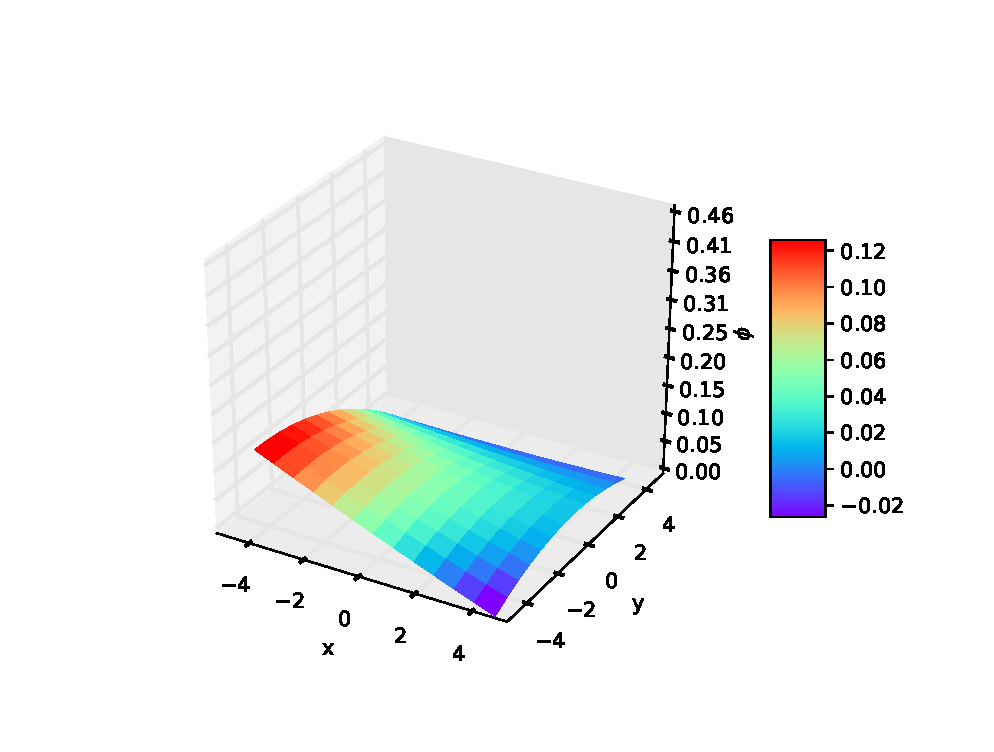
\includegraphics[width=1.0\linewidth]{figure/figureR}
	\caption{矩形边界接地内部点电荷电势分布}
	\label{fig:figureR}
	\end{figure}
	\begin{figure}[h]
		\centering
		\includegraphics[width=1.0\linewidth]{figure/figure5}
		\caption{矩形边界接地内部点电荷电势分布}
		\label{fig:figure5}
	\end{figure}
		

	由于使用2次幂级数拟合使得电势分布相对平滑,并不特别符合物理事实,所以使用Matlab中的Curve fitting工具进行拟合,矩形边界条件电势分布见Figure 5。观察图像可以发现电势最高点为(-3.5,-2.0)位置附近,其余位置的电势近似成负幂次衰减,因此得出结论:有限差分法求解矩形边界条件Poisson方程得到的解较为符合物理认识,并且整个图像较为合理。
	
	
	在(2,0)位置处(可以在生成矩阵的程序修改x0,y0参数从而改变位置,见附录B)放置一个点电荷,这里点电荷我们直接用1代替,求解矩阵大小为170,则可以求解出电势随坐标分布见Figure 6。
	\begin{figure}[h]
		\centering
		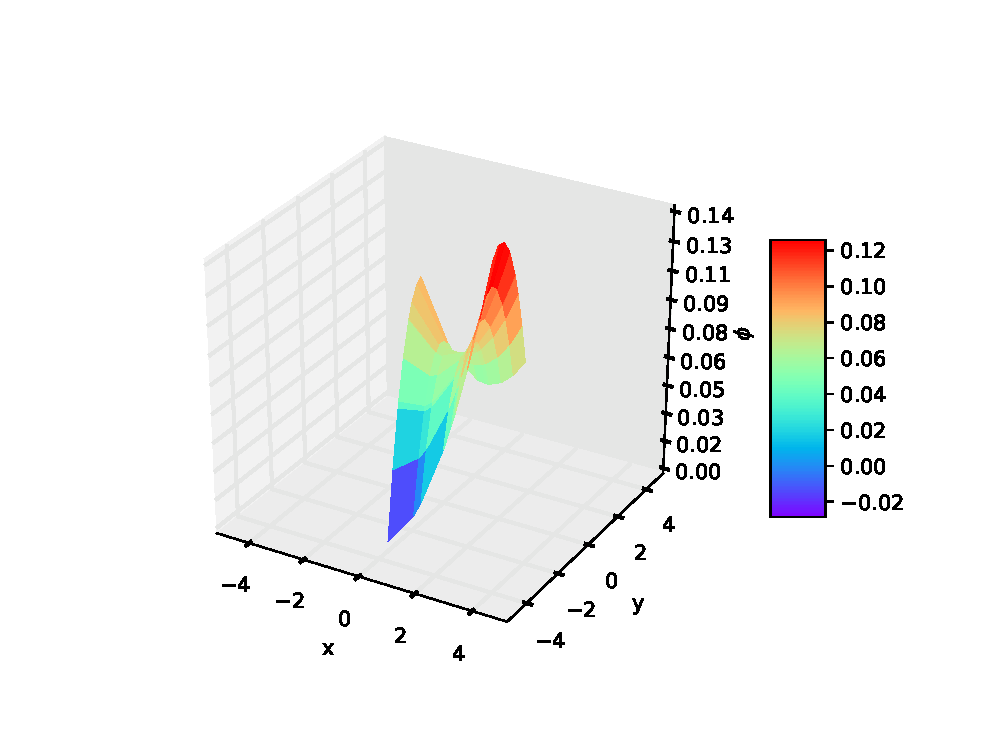
\includegraphics[width=1.0\linewidth]{figure/figureC}
		\caption{圆形边界接地内部点电荷电势分布}
		\label{fig:figureC}
	\end{figure}
	
	同样使用Matlab中的Curve fitting工具进行拟合,极坐标边界条件电势分布见Figure 7。
	\begin{figure}[h]
		\centering
		\includegraphics[width=1.0\linewidth]{figure/figure7}
		\caption{圆形边界接地内部点电荷电势分布}
		\label{fig:figure7}
	\end{figure}	
	\onecolumn
	为了对各种求解线性方程组的方法进行计算速度分析,我们统计了不同算法处理相同矩阵的运行时间,见Figure 8和Figure 9。
	\begin{figure}[h]
	\centering
	\includegraphics[width=0.6\linewidth]{figure/timeR}
	\caption{矩形边界下不同算法计算速度分析}
	\label{fig:timeR}
	\end{figure}	
	\begin{figure}[h]
		\centering
		\includegraphics[width=0.6\linewidth]{figure/timeC}
		\caption{圆形边界下不同算法计算速度分析}
		\label{fig:timeC}
	\end{figure}	
	
	由于采用了Python time宏包内部的time.clock()函数,可能对于记录时间一问题处理并不是特别完美,可以看到曲线可能会存在波动,但是总体可以看出,不同求解线性方程组的方法中计算速度从快到慢依次为:SOR超松弛迭代法、Gauss Seidel迭代法、Jacobi迭代法、Gauss消元法。
	
%----------------------------------------------------------------------------------------
%	APPENDICES SECTION
%----------------------------------------------------------------------------------------

\newpage
\onecolumn
\begin{appendices}
\section{矩形边界生成Cartesian坐标下有限差分格式矩阵}
矩形边界生成Cartesian坐标下有限差分格式矩阵,为了可以不断扩大矩阵尺寸,我们将不同大小的线性方程组分别存到Rmatrix.xlsx工作簿的不同Sheet表格中。\\
\textbf{\textcolor[rgb]{0.98,0.00,0.00}{Input Python source:}}
\lstinputlisting[language=Python]{./program/Rectangle_Poisson.py}
\newpage
\section{圆形边界生成极坐标下有限差分格式矩阵}
圆形边界生成极坐标下有限差分格式矩阵,为了可以不断扩大矩阵尺寸,我们将不同大小的线性方程组分别存到Cmatrix.xlsx工作簿的不同Sheet表格中。\\
\textbf{\textcolor[rgb]{0.98,0.00,0.00}{Input Python source:}}
\lstinputlisting[language=Python]{./program/Circle_Poisson.py}
\newpage
\section{不同求解线性方程组的方法}
将求解线性方程组的方法分别写成子函数合在一起写成一个叫做method.py的Python程序,方便调用。\\
\textbf{\textcolor[rgb]{0.98,0.00,0.00}{Input Python source:}}
\lstinputlisting[language=Python]{./program/method.py}
\newpage
\section{计算分析绘图}
通过读取Rmatrix.xlsx和Cmatrix.xlsx文件中的矩阵数据,并调用上述子函数分别进行运算,我们可以绘制出不同大小矩阵的Cartesian坐标下矩形边界内部有一个点电荷的导体接地的Poisson方程及极坐标下圆形边界内部有一个点电荷的导体接地的Poisson方程的解,这里为了展示方便,只绘制选定最大限度的矩阵的情况。\\
\textbf{\textcolor[rgb]{0.98,0.00,0.00}{Input Python source:}}
\lstinputlisting[language=Python]{./program/draw1.py}
\newpage
\section{计算分析绘图}
通过读取Rmatrix.xlsx和Cmatrix.xlsx文件中的矩阵数据,并调用上述子函数分别进行运算,通过统计不同算法的运行时间,我们可以绘制出不同算法运行时间与矩阵大小的关系。\\
\textbf{\textcolor[rgb]{0.98,0.00,0.00}{Input Python source:}}
\lstinputlisting[language=Python]{./program/draw2.py}
\end{appendices}

%----------------------------------------------------------------------------------------
%	REFERENCE
%----------------------------------------------------------------------------------------

\newpage
\renewcommand\refname{参考文献}
\begin{thebibliography}{99}
\bibitem{ref1} Jackson, Julia A.; Mehl, James P.; Neuendorf, Klaus K. E. (编), Glossary of Geology, American Geological Institute, Springer: 503, 2005, ISBN 9780922152766.
\bibitem{ref2}Poisson Equation at EqWorld: The World of Mathematical Equations.
\bibitem{ref3}L.C. Evans, Partial Differential Equations, American Mathematical Society, Providence, 1998. ISBN 0-8218-0772-2.
\bibitem{ref4}A. D. Polyanin, Handbook of Linear Partial Differential Equations for Engineers and Scientists, Chapman \& Hall/CRC Press, Boca Raton, 2002. ISBN 1-58488-299-9.
\bibitem{ref5}Crank, J. The Mathematics of Diffusion. 2nd Edition, Oxford, 1975, p. 143.
\bibitem{ref6}K.W. Morton and D.F. Mayers, Numerical Solution of Partial Differential Equations, An Introduction. Cambridge University Press, 2005.
\bibitem{ref7}Oliver Rübenkönig, The Finite Difference Method (FDM) - An introduction, (2006) Albert Ludwigs University of Freiburg.
\bibitem{ref8}Autar Kaw and E. Eric Kalu, Numerical Methods with Applications, (2008).
\bibitem{ref9} 第八章 方程,《九章算术》.
\bibitem{ref10}Atkinson, Kendall A. An Introduction to Numerical Analysis, 第二版, John Wiley \& Sons, New York, 1989年 ISBN 978-0-471-50023-0.
\bibitem{ref11}Golub, Gene H., and Van Loan, Charles F. Matrix computations, 第三版, Johns Hopkins, Baltimore, 1996年 ISBN 978-0-8018-5414-9.
\bibitem{ref12}Black, Noel; Moore, Shirley; and Weisstein, Eric W. Jacobi method. MathWorld.
\bibitem{ref13}A. Hadjidimos, Successive overrelaxation (SOR) and related methods, Journal of Computational and Applied Mathematics 123 (2000), 177-199.
\bibitem{ref14}Yousef Saad, Iterative Methods for Sparse Linear Systems, 1st edition, PWS, 1996.
\bibitem{ref15}
Netlib's copy of "Templates for the Solution of Linear Systems", by Barrett et al.
\bibitem{ref16}.
Richard S. Varga 2002 Matrix Iterative Analysis, Second ed. (of 1962 Prentice Hall edition), Springer-Verlag.
\bibitem{ref17}
David M. Young, Jr. Iterative Solution of Large Linear Systems, Academic Press, 1971. (reprinted by Dover, 2003)
\end{thebibliography} 

%----------------------------------------------------------------------------------------
\end{CJK*}
\end{document}
